\nonstopmode
\documentclass{article}
\usepackage[utf8]{inputenc}
\usepackage{graphicx}
\graphicspath{ {images/} }
\usepackage{polski}
\usepackage{subcaption}

\title{Sprawozdanie z algorytmów sortowania}
\author{Adam Piaseczny, Igor Szczepaniak}
\date{Marzec 2022}

\begin{document}

\maketitle
\pagebreak

\tableofcontents
\pagebreak

\section{Wprowadzenie}
W tym sprawozdaniu porównaliśmy ze sobą osiem różnych algorytmów sortowania w zróżnicowanych warunkach i przy określonych ilościach danych w nich zawartych. Analizując wyniki otrzymane podczas doświadczenia byliśmy w stanie sprawdzić w kontrolowanym środowisku, jakie są właściwości poszczególnych algorytmów i jak może to pomóc zastosowaniu ich w praktyce. Cały program został napisany w języku \verb+python+ z powodu prostoty implementacji funkcji testujących.
\subsection{Generator tablic}

Z racji powolnej natury list w języku \verb+python+, postanowiliśmy użyć biblioteki \verb+numpy+ jako głównego narzędzia do generowania tablic. Pomogło to znacznie w procesie tworzenia pseudolosowych rozkładów liczb oraz ich analizie.

\section{Analiza zadań}

Do wykonania było zadanych łącznie 7 testów. Trzy z zadnia drugiego, dwa z trzeciego oraz dwa z czwartego.

\subsection{Pierwszy test - wszystkie algorytmy}

W tym teście zawarliśmy 20 prób, z wartościami $n$ od 1000 do 20000 w rozkładzie losowym dla następujących prostych algorytmów sortowania:

\begin{enumerate}
    \item Selection Sort
    \item Insertion Sort
    \item Bubble Sort
\end{enumerate}

Oraz dla czterech złożonych:

\begin{enumerate}
    \item Heap Sort
    \item Merge Sort
    \item Counting Sort
    \item Quicksort z podziałem według środkowego elementu
\end{enumerate}

\newpage

\subsubsection{Rozkład losowy}

Z racji dużych różnic w czasie wykonywania zrobiliśmy dwa osobne wykresy dla poszczególnych kategorii. Dane dla algorytmów prostych są zawarte w wykresie nr 1, a dla złożonych w wykresie nr 2.

\begin{figure}[h]
\centering
\begin{minipage}{.5\textwidth}
  \centering
  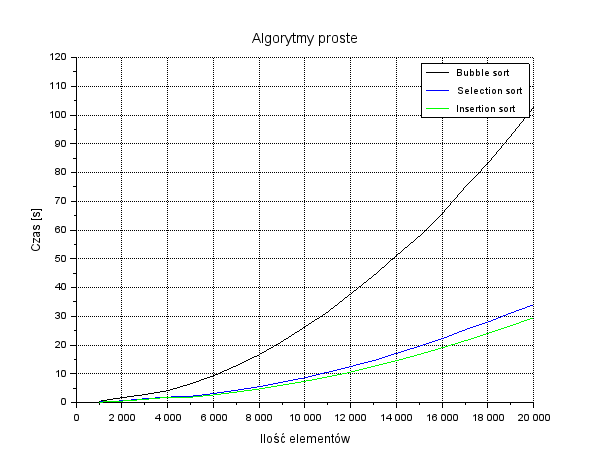
\includegraphics[width=1\linewidth]{proste}
  \captionof{figure}{$t=f(n)$ - proste}
  \label{fig:proste}
\end{minipage}%
\begin{minipage}{.5\textwidth}
  \centering
  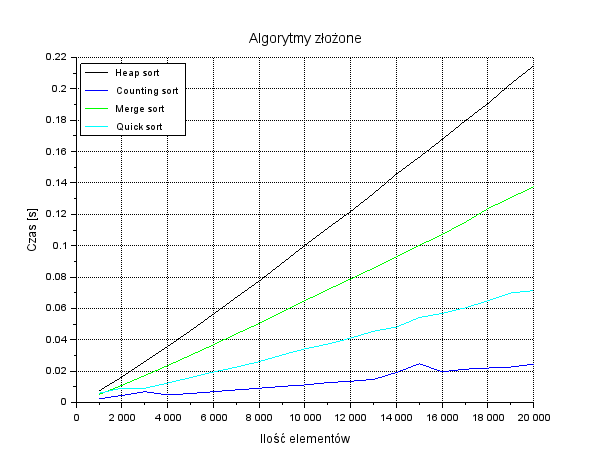
\includegraphics[width=1\linewidth]{zlozone}
  \captionof{figure}{$t=f(n)$ - złożone}
  \label{fig:zlozone}
\end{minipage}
\end{figure}

Analizując wykresy zauważyliśmy, że czas pracy algorytmów prostych znacznie odbiega od złożonych. Nie jest to zaskakujące, znając żłożoność obliczeniową tych algorytmów w przypadku średnim. Wykres pokazuje w sposób graficzny, jak bardzo różnią się te algorytmy, widać to po samej skali w jakiej rozpatrywane są wyniki.

\subsubsection{Rozkład rosnący}

Przy rozkładzie rosnącym (posortowanej tablicy) od razu zauważamy, że Bubble Sort, który w poprzedniej próbie wypadł najgorzej, zakończył swoje wykonywanie w rekordowym czasie, ponieważ implementacja naszego algorytmu przewidywuje tzw. "flagę", która pozwala szybko wykryć częściowe posortowanie tablicy wejściowej.

\begin{figure}[h]
\centering
\begin{minipage}{.5\textwidth}
  \centering
  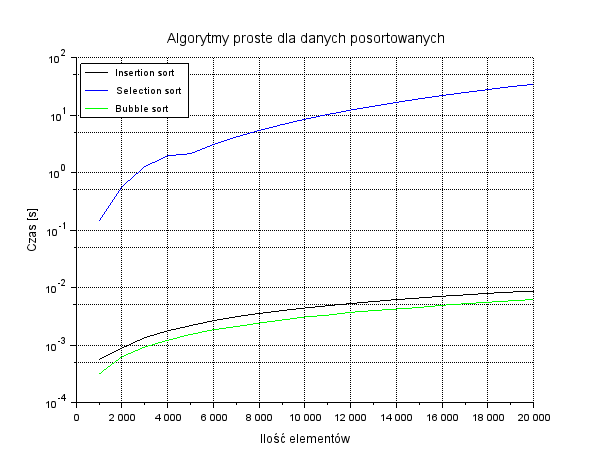
\includegraphics[width=1\linewidth]{proste posortowane.png}
  \captionof{figure}{$t=f(n)$ - proste}
  \label{fig:proste_sorted}
\end{minipage}%
\begin{minipage}{.5\textwidth}
  \centering
  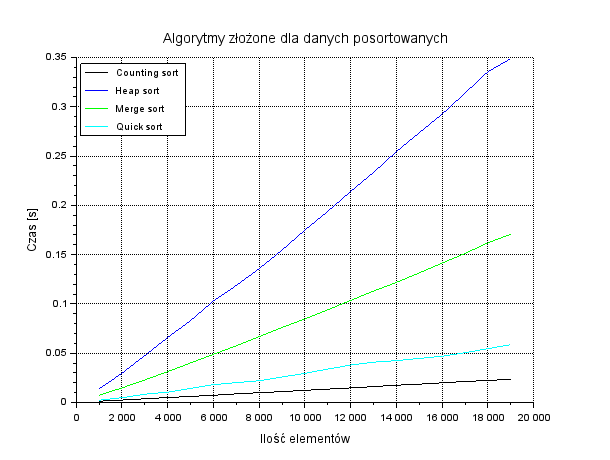
\includegraphics[width=1\linewidth]{zlozone posortowane.png}
  \captionof{figure}{$t=f(n)$ - złożone}
  \label{fig:zlozone posortowane}
\end{minipage}
\end{figure}

\subsubsection{Rozkład malejący}
Przy rozkładzie malejącym (tablicy odwrotnie posortowanej) zauważamy najgorszy przypadek dla algorytmów selection oraz bubble sort.

\begin{figure}[h]
\centering
\begin{minipage}{.5\textwidth}
  \centering
  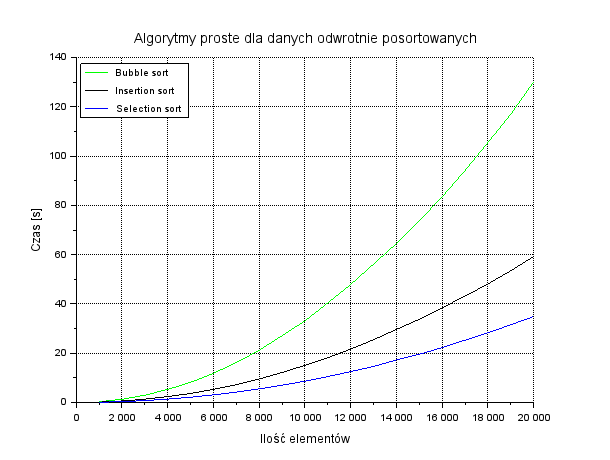
\includegraphics[width=1\linewidth]{proste odwrotnie posortowane.png}
  \captionof{figure}{$t=f(n)$ - proste}
  \label{fig:proste_reverse_sorted}
\end{minipage}%
\begin{minipage}{.5\textwidth}
  \centering
  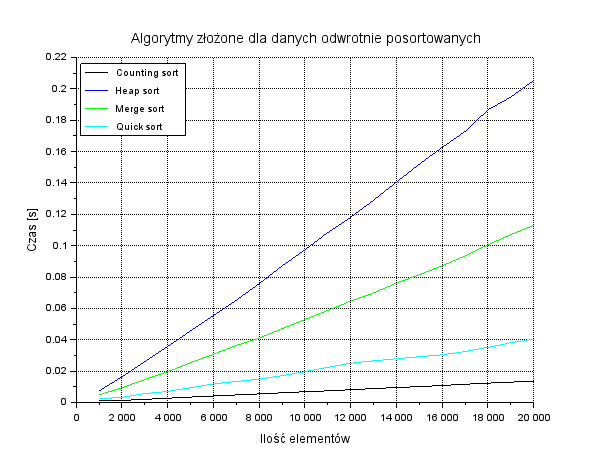
\includegraphics[width=1\linewidth]{zlozone odwrotnie posortowane.png}
  \captionof{figure}{$t=f(n)$ - złożone}
  \label{fig:zlozone_odwrotnie_posoortwane}
\end{minipage}
\end{figure}

\subsubsection{Wnioski}

Z wykonanych testów byliśmy w stanie potwierdzić, jakie są najgorsze oraz najlepsze przypadki dla poszczególnych algorytmów sortowania i dowiedzieć się, kiedy najlepiej ich używać w praktyce. Metody proste zwykle nie są efektywne dla dużej ilości danych lecz dla wszystkich istnieje zastosowanie. Dla każdego przypadku wypisaliśmy najlepszy według nas użytek dla danego algorytmu.

\begin{enumerate}
	\item Insertion Sort - kiedy $n$ jest małe
	\item Selection Sort - kiedy potrzebna jest szybka implementacja
	\item Bubble Sort - w przypadku prawie posortowanych tablic, dodatkowym atutem jest łatwość implementacji
	\item Heap Sort - kiedy potrzebny jest stabilny algorytm i mamy ograniczony z góry czas
	\item Merge Sort - kiedy potrzebne jest stabilne sortowanie $O(n\log n)$
	\item Counting Sort - kiedy sortujemy liczby całkowite o małej rozpiętości
	\item Quicksort (\verb+pivot+ na środku) - kiedy potrzeba szybkiego sortowania i średni przypadek ma duże znaczenie

\end{enumerate}

\subsection{Drugi test - szybkie oraz wstawanie}

Tutaj porównane będą dwie wersje algorytmu Quick Sort (z podziałem według skrajnego i środkowego elementu tablicy) wraz z algorytmem sortowania przez proste wstawianie. Nasze testy są w zakresie wartości $n$ od 300 do 3000 włącznie.

\subsubsection{Rozkład losowy i rosnący}

Przy rozkładzie losowym obie wersje Quick Sort mają porównywalne czasy wykonania, o wiele szybsze od sortowania przez proste wstawianie. Natomiast przy rozkładzie rosnącym zauważamy znaczne pogorszenie czasu obu sortowań szybkich, które w tym teście wypadają dużo gorzej niż prosty algorytm przez wstawianie. Warto zaznaczyć, że Quick Sort z podziałem według elementu skrajnego ma znacznie większy czas pracy niż wersja z elementem środkowym.

\begin{figure}[h]
\centering
\begin{minipage}{.5\textwidth}
  \centering
  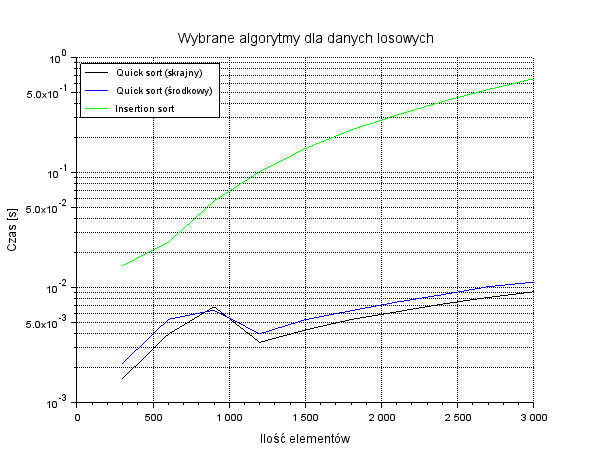
\includegraphics[width=1\linewidth]{losowe}
				\captionof{figure}{Rozkład losowy}
  \label{fig:losowe}
\end{minipage}%
\begin{minipage}{.5\textwidth}
  \centering
				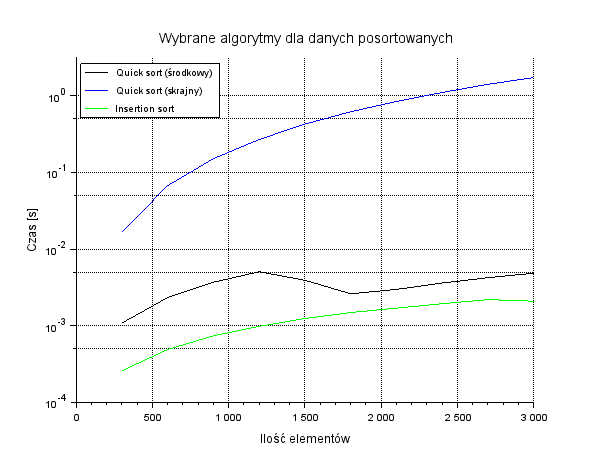
\includegraphics[width=1\linewidth]{posortowane}
  \captionof{figure}{Rozkład rosnący}
  \label{fig:rozklad_rosnacy}
\end{minipage}
\end{figure}

\subsubsection{Wnioski}

Duży czas pracy sortowania z elementem skrajnym w przypadku dla danych rosnących jest wynikiem, rekurencyjnego wykonywania funkcji aż $n-1$ razy. Napotykając ten problem, byliśmy zmuszeni obniżyć wartości $n$ w poszczególnych testach, jak również zwiększyć limit stosu rekurencyjnego. W tym właśnie przypadku sortowanie szybkie zajmowało skrajnie dużo pamięci, co było znacznym problemem w procesie sprawdzania jego zachowania.

W implementacji algorytmu Quick Sort niezbędne jest zastanowienie się nad sposobem wyboru elementu \verb+pivot+, widząc jak bardzo wpływa on na efektywność algorytmu i jego najgorszy przypadek. Wybieranie tego elementu jako losowego w tablicy minimalizuje możliwość najgorszego przypadku, popularnym rozwiązaniem jest również wybranie trzech losowych indeksów i wybranie tego, który jest środkowym.

Metoda Insertion Sort jest zwykle wolniejsza od sortowania szybkiego, lecz ważnym faktem jest to, że jej najgorszy oraz średni najlepszy przypadek mają taką samą złożoność czasową, a najlepszy ma złożoność $O(n)$ co przydaje się mając prawie posortowane dane. Sortowanie przez wstawianie również nie wymaga dodatkowego nakładu pamięci - wykonuje się "w miejscu" podczas gdy sortowanie szybkie potrafi pochłonąć prawie cały stos rekurencyjny w najgorszym przypadku i jest bardzo zachłanny w kontekście pamięci. Quick Sort dla średniego przypadku jest za to o wiele bardziej efektywny i ma bardziej ogólne zastosowanie.

\subsection{Trzeci test - rozpiętość przedziałowa danych}

W tym teście sprawdzamy jak zachowują się dwa algorytmy - Counting Sort oraz Quick Sort (z podziałem środkowym) dla wartości $n$ od 1000 do 20000 mając 20 puktów pomiarowych. Za to zakres wartości znacząco różni się miedzy testami.

\subsubsection{Przentacja danych}

Na pierwszym wykresie zakres danych mieści się w zakresie $[1,100*n]$, na drugim za to widzimy zależność przy zakresie $[1,0.01*n]$.

\begin{figure}[h]
\centering
\begin{minipage}{.5\textwidth}
  \centering
  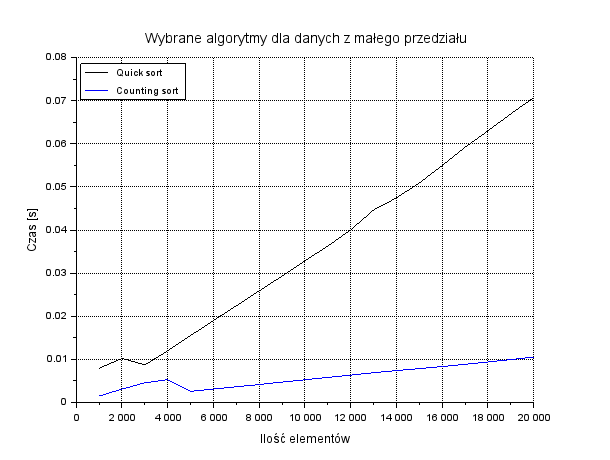
\includegraphics[width=1\linewidth]{male}
  \captionof{figure}{Mała rozpiętość danych}
  \label{fig:male}
\end{minipage}%
\begin{minipage}{.5\textwidth}
  \centering
				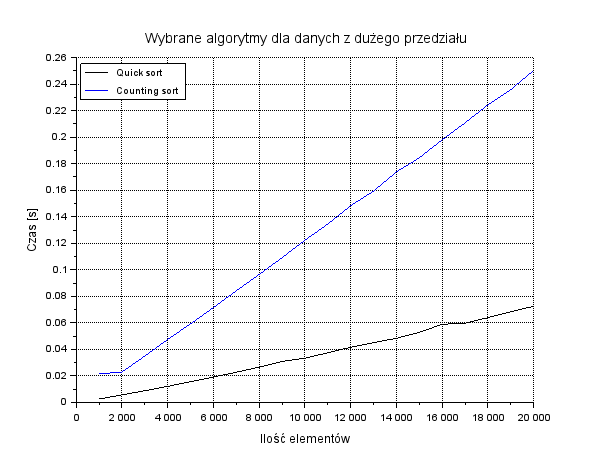
\includegraphics[width=1\linewidth]{duze}
  \captionof{figure}{Duża rozpiętość danych}
  \label{fig:duze}
\end{minipage}
\end{figure}

\subsubsection{Wnioski}

Na pierwszym wykresie w konteście czasu wykonania przoduje Quick Sort, lepiej radząc sobie z dużą rozpiętością analizowanych danych, za to Counting Sort z powodu zasady swojego działania ma możliwość pokazania swojej "szybkiej strony" przy małej rozpiętości danych. Dzieje się tak z racji tworzenia mniejszej tablicy pomocniczej i operowania na niej. Warto również zauważyć, że rozpiętość danych prawie w ogóle nie wpływa na szybkość działania sortowania szybkiego, podczas gdy w sortowaniu przez zliczanie zauważamy ogromną różnicę. Przy doborze metod sortowania zależy dokładnie przyjrzeć się zakresowi rozpatrywanych danych, aby na pewno nie przeoczyć lepszego rozwiązania.

\section{Podsumowanie}

W sprawozdaniu porównaliśmy i przeanalizowaliśmy różne algorytmy sortujące, pokazaliśmy ich dobre i złe strony oraz jak zachowują się w poszczególnych warunkach w kontrolowanym środowisku. Kod do wykorzystanego programu oraz pliki z danymi wyjściowymi dostępne są pod następującą witryną: \\\\
https://github.com/TypicalAM/Sorting-Algorithms

\end{document}

